\documentclass[conference]{IEEEtran}
\IEEEoverridecommandlockouts
% The preceding line is only needed to identify funding in the first footnote. If that is unneeded, please comment it out.
\usepackage{cite}
\usepackage{amsmath,amssymb,amsfonts}
\usepackage{algorithmic}
\usepackage{graphicx}
\usepackage{textcomp}
\usepackage{xcolor}
\usepackage{caption}
\usepackage{subcaption}
\usepackage{array}
\usepackage{pgf-pie} %for pie chart
\graphicspath{ {./fig/} }
\usepackage{mathtools} 

%added by Ye
\usepackage{fontspec}

%for typing Myanmar text, you can also used with Myanmar3 font
\newfontfamily {\padauktext}[Script=Myanmar]{Padauk}
%\newfontinstance {\padauktext}[Script=Myanmar]{Padauk}

%for double quote
\newcommand{\quotes}[1]{``#1''}
\renewcommand{\baselinestretch}{0.86}
%added by Ye

\def\BibTeX{{\rm B\kern-.05em{\sc i\kern-.025em b}\kern-.08em
    T\kern-.1667em\lower.7ex\hbox{E}\kern-.125emX}}
\begin{document}

\title{University of Technology(Yatanarpon Cyber City)}

\author{\IEEEauthorblockN{Myo Mar Thinn}
\IEEEauthorblockA{\textit{B.E(Information Science and Technology)} \\
\textit{myomarthinnutycc96@gmail.com}
}
}

\maketitle

\begin{abstract}
University of Technology (Yatanarpon Cyber City) namely UTYCC is a speedy developing learning community that has been recognized as one of the most Myanmar’s technological institutions of higher education. Although it is founded in 2010, UTYCC becomes very well-known both locally and globally within a short period of time.\\
There are four main faculties in our university: Faculty of Information \& Communication Technology, Faculty of Electronic Engineering, Faculty of Precision Engineering and Faculty of Materials Engineering. As UTYCC intends to foster best knowledge and bright future with the high level of innovation, many talented students are interested in it and enroll every year. The sports and recreation activities throughout the academic year are also one main attraction for the new students. The university is located in the best climate area.\\
As an international collaboration program, UTYCC is a member institute of ASEAN Cyber University Project. E-learning center was established with the assistance of Korea International Cooperation Agency (KOICA) in July 2012. Since then, online contents are being developed every academic year. Moreover, there is Double Master Degree Program with University of Miyazaki, Japan. In order to achieve the work readiness skills of the students, the university provides internship programs for the students with the link of industry partners and collaborates with Mekong Skills to work USAID Project..
\end{abstract}

\section{Academic Programmes}
The University aims to provide higher quality education. A wide range of undergraduate and postgraduate degree programmes are offered in this university.
\subsection{Bachelor Programme}
The bachelor degree program is a foundation programme and challenging for the preparation of young individuals who are able to fulfill ever-changing demand of 21st century education. With a variety of courses offered by the various faculties, the candidate will benefit from a broad-based education in multiple disciplines.

The candidate who wants to join bachelor degree programme must pass the matriculation exam held by the government and must have the total exam marks at least 420.

To achieve a Bachelor Degree, students have to attend six years. There are two semesters in an academic year. For each semester, it includes mid-term and final exams, tutorials, case study, practical/lab tests and project according to the nature of subject. The students must have at least 75\% attendance in every lecture for taking exam. The students will achieve the degree unless they fail to submit mini-thesis in the final year. 
The Bachelor Degree programmes are:
\begin{itemize}
 \item B.E (Information Science and Technology)
 \item B.E (Computer Engineering)
 \item B.E (Electronics)
 \item B.E (Materials and Metallurgy)
 \item B.E (Mechanical Precision and Automation)
\end{itemize}

\subsection{Master Programme (M.E)}
Master degree programme provides the advanced skills and research needed to work as a qualified engineer in specific specialized-areas. It encompasses the latest research for the development of society and solving the real world problems.

The student who wants to join master degree programme must possess a bachelor degree in engineering passed with credit in a specific field. Students are required to take the entrance exam and oral test. The students who pass the entrance exam and oral test can join the master degree programme. They are required to attend one year course work and one year thesis.

The master degree programmes are:
\begin{itemize}
\item M.E (Information Science and Technology)
\item M.E (Computer Engineering)
\item M.E (Electronics)
\item M.E (Materials and Metallurgy)
\item M.E (Mechanical Precision and Automation)
\end{itemize}

\subsection{Doctorate Programme (Ph.D)}
The university provides doctor of philosophy in Information Technology degree programme which is a starting point in earning the lifelong task of learning how to do research and academic life. The candidates should be curious to find out the unknown facts of an event and new things. Their research should be able to serve the society by solving social problems. If the candidates want to join this program, the candidates must require the successful completion of master degree and they must take the entrance exam and oral test. They have to study course work for one year and do research work for two years in minimum. The candidates must achieve the successful completion of the course work and research. After the research has been successfully completed, they will get Ph.D. (Information Technology). The doctoral degree program currently offered in our university is:
\begin{itemize}
\item Ph.D (Information Technology)
\end{itemize}

\section{About}
There are four faculties and five departments.
\begin{itemize}
\item Faculties
\begin{itemize}
\item Faculty of Information and Communication Technology
\begin{itemize}
\item Department of Information Science
\item Department of Computer Engineering
\end{itemize}
\item Faculty of Electronics Engineering
\item Faculty of Advanced Material Engineering
\item Faculty of Precision Engineering
\end{itemize}
\item Departments
\begin{itemize}
\item Department of Myanmar
\item Department of English
\item Department of Engineering Mathematics
\item Department of Engineering Physics
\item Department of Engineering Chemistry
\end{itemize}
\item QMS Department
\item IR Department
\item Learning Center
\begin{itemize}
\item ASEAN Cyber University Project e-learning Center
\item Mekong Learning Center (USAID COMET)
\end{itemize}
\end{itemize}
The follwing chart shows number of Students in each faculty \bf{(2016-2017)}.\\

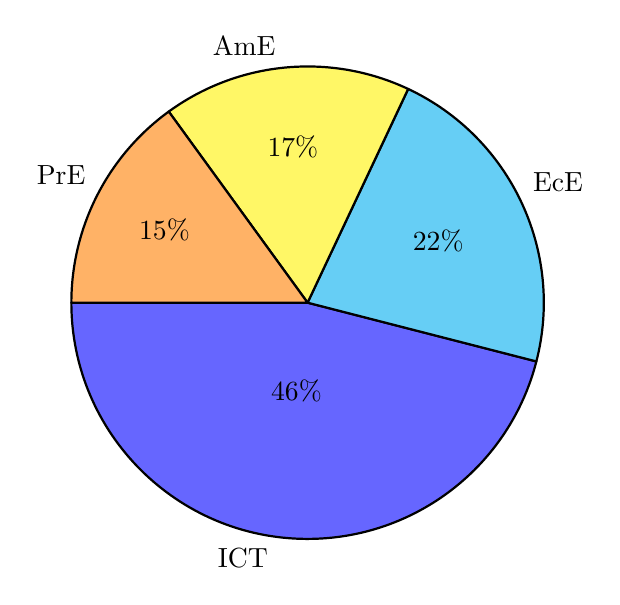
\begin{tikzpicture}
\pie [rotate = 180]
    {46/ICT,22/EcE,17/AmE,15/PrE}
\end{tikzpicture}


\begin{table}[h!]
\caption{\label{table:RawangKachinCM} Student List in each academic \bf{2016-2017}}

\begin{center}
\begin{tabular}{ |c|c| } 
 \hline
 \bf Academic & \bf No of Students \\ [5pt]
 \hline
 Undergraduate  & 1399 \\[5pt]
 \hline
 Master  & 85 \\[5pt]
 \hline
 Ph.D (IT) (Course Work) & 85 \\[5pt]
 \hline
 International Students  & 3 \\[5pt]
 \hline
\end{tabular}
\end{center}
\end{table}

\section{Faculities}
\subsection{Faculty of Information and Communication Technology}
Faculty of Information and Communication Technology of University of Technology (Yatanarpon Cyber City) is organized with competent instructors and enthusiastic researchers. We educate the students to be talented in their study areas and conduct innovative scientific research.\\
The students are being trained to have 21st century skills comprised of: collaboration and team work skills, creativity and imagination skills, critical thinking and problem solving skills. Due to their in-depth knowledge of information science and computer engineering, they are able to solve the real world problems faced within society in sophisticated way that lead to achieve work readiness skills. The Faculty is composed of two sub-departments.
\subsubsection{Department of Information Science}
Department of Information Science is recognized as one of the most prominent departments for theoretical and methodological reflection of computer science and information practice. The department is preparing the future generations of information specialists for managing communication flows, support of knowledge economy and handling the information explosion. Highly qualified instructors are exploring and doing research that contributes to the society by collaborating with Master and Ph.D. candidates.\\
The department encourages instructors’ involvement within the contemporary business world to enhance the quality of classroom instruction and contribute to students’ learning. After completing the study, students are capable of joining multinational companies in IT industry.
\\
\begin{itemize}
\item Vision\\ \\
\noindent\fbox{%
    \parbox[c][10mm][c]{80mm}{%
        \begin{itemize}
	\item To become intellectual professional, practitioners and future leaders of emerging information technologies
	\end{itemize}
    }%
}
\\ \\
\item Mission\\ \\
\noindent\fbox{%
    \parbox[c][35mm][c]{80mm}{%
        \begin{itemize}
	\item To train the students to become innovators with best standard of theoretical and practical aspects of emerging information 		technology and a user community
        \item To provide the students in order to solve the challenging real-world problems with the effectively use of the most innovative 		technology
        \item To provide wide access of learning environment with the application of ICT
	\end{itemize}
    }%
}
\\ \\
\item Motto\\ \\
\noindent\fbox{%
    \parbox[c][7mm][c]{80mm}{%
        \begin{itemize}
	\item To Build a Better Society Through ICT
	\end{itemize}
    }%
}
\end{itemize}
\subsubsection{Department of Computer Engineering}
 Computer Engineering Department offers high quality engineering education equipped with state of the art knowledge and skills to the students in order to become life-long learners, problem solvers and engineers with the scene of professional responsibility. The courses from our Department cover communication network, network security, embedded system and IoT. AI and Machine Learning and other ICT engineering related. These courses are delivered by highly qualified faculty members as well as researchers.
\subsection{Faculty of Precision Engineering}
Precision engineering and manufacturing issues are becoming ever more important in current and future technologies. Precision engineering is defined as painstaking attention to details and requires knowledge of a wide variety of measurement, fabrication, and control issues. Precision manufacturing is defined as the manufacture of individual pieces with extreme accuracy. This type of machining is used to make parts for various machines, including medical, aeronautical, and any other industry that requires identical parts to be created in large quantities.\\
Precision engineering is a sub-discipline of mechanical engineering, electrical engineering, software engineering, electrical engineering, control engineering, and optical engineering. It is concerned with designing machines, fixture, and other structures that have exceptionally high tolerances, are repeatable, and are stable over time. This engineering field will aid in the advancement of various technologies that need to gain industrial competitiveness.
\subsection{Faculty of Advanced Material Engineering}
Materials that are utilized in high-technology applications are termed advanced materials. By high technology we mean a device or product that operates or functions using relatively intricate and sophisticated principles; examples include electronic equipment, computers, fiber-optic systems, spacecraft, aircraft, and military rocketry. These advanced materials are typically traditional materials whose properties have been enhanced, and, also newly developed, high-performance materials. Furthermore, they may be of all material types, and are normally expensive. Advanced materials include semiconductors, biomaterials, and “materials of the future” (that is, smart materials and nanoengineered materials). The properties and applications of a number of these advanced materials - for example, materials that are used for lasers, integrated circuits, magnetic information storage, liquid crystal displays (LCDs), and fiber optics need to study.\\
Processing, Structure, Properties and Performance are the main discipline of materials science and engineering and their interrelationship. There is a recognized need to find new, economical sources of energy and to use present resources more efficiently. Materials will undoubtedly play a significant role in these developments.

\section{Head of University}

\begin{figure}[h]
\centering
\includegraphics[width=5cm, height=5cm]{sayar}
\caption{Head of University}
\end{figure}
\begin{itemize}
\item Dr.Aung Win
\item Rector (Acting), University of Technology (Yatanarpon Cyber City)
\item Ph.D (IT)
\item dr.aungwin@utycc.edu.mm
\item most.yatanarpon@gmail.com
\end{itemize}

\section*{Contact Us}
\noindent\fbox{%
    \parbox[c][25mm][c]{90mm}{%
        \begin{itemize}
	\item +95-025178100, +95-025178200, +95-025178103
        \item info@utycc.edu.mm
        \item At 28 miles on Mandalay – Lashio road, between Pyin Sar Village and Thone Taung Village, Pyin Oo Lwin, Myanmar.
	\end{itemize}
    }%
}

\end{document}
